% Standalone Paper 1 figures; values are derived from artifacts/stage7/pilot_validation.json.
\newcommand{\figPaperOneArchitecture}{%
\begin{figure*}[t]
\centering
\resizebox{\textwidth}{!}{%
\begin{tikzpicture}[font=\footnotesize,node distance=8mm and 10mm,
box/.style={draw,rounded corners,align=center,minimum height=9mm,minimum width=31mm},
small/.style={draw,rounded corners,align=center,minimum height=8mm,minimum width=29mm},
arr/.style={-Latex,thick}]
\node[box] (state) {Vehicular state\\$R$, $v$, SNR, Doppler};
\node[box,right=of state] (profile) {Waveform profile\\$B,T_c,T_r,F_s$};
\node[box,right=of profile] (cap) {Capability derivation\\$\Delta R,R_{\max},\Delta v,v_{\max}$};
\node[box,right=of cap] (gate) {Deterministic\\physics gate};
\node[box,right=of gate] (action) {54-action PHY\\configuration set};
\node[small,below=of action,xshift=-17mm] (comm) {One-way communication\\dechirp + DBPSK};
\node[small,below=of action,xshift=17mm] (sens) {Two-way monostatic sensing\\IF + range--Doppler};
\draw[arr](state)--(profile);
\draw[arr](profile)--(cap);
\draw[arr](cap)--(gate);
\draw[arr](gate)--(action);
\draw[arr](action)--(comm);
\draw[arr](action)--(sens);
\end{tikzpicture}%
}%
\caption{Paper 1 architecture. Profile-level physical capability is derived before configuration selection. The communication path is one-way, while the sensing echo is two-way monostatic and processed at dechirped IF.}
\label{fig:p1architecture}
\end{figure*}%
}

\newcommand{\figPaper1Capability}{%
\begin{figure}[t]
\centering
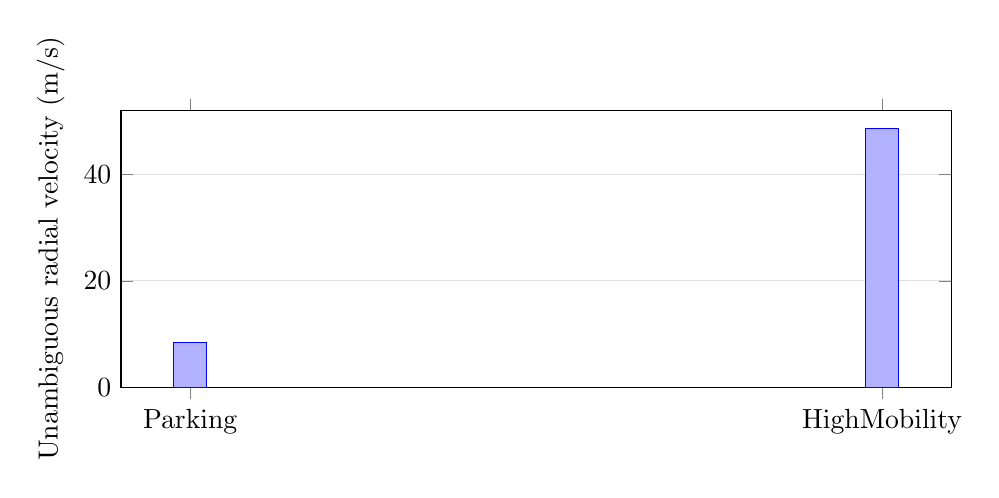
\begin{tikzpicture}
\begin{axis}[
width=\columnwidth,height=5.1cm,
ybar,bar width=12pt,ymin=0,ymax=52,
ylabel={Unambiguous radial velocity (m/s)},
symbolic x coords={Parking,HighMobility},xtick=data,
ymajorgrids=true,grid style={black!12}]
\addplot coordinates {(Parking,8.4055)(HighMobility,48.6676)};
\end{axis}
\end{tikzpicture}
\caption{Derived monostatic unambiguous radial-velocity support. The high-mobility capability profile extends the support by a factor of approximately 5.79 relative to the parking profile.}
\label{fig:p1capability}
\end{figure}%
}

\newcommand{\figPaper1Pilot}{%
\begin{figure*}[t]
\centering
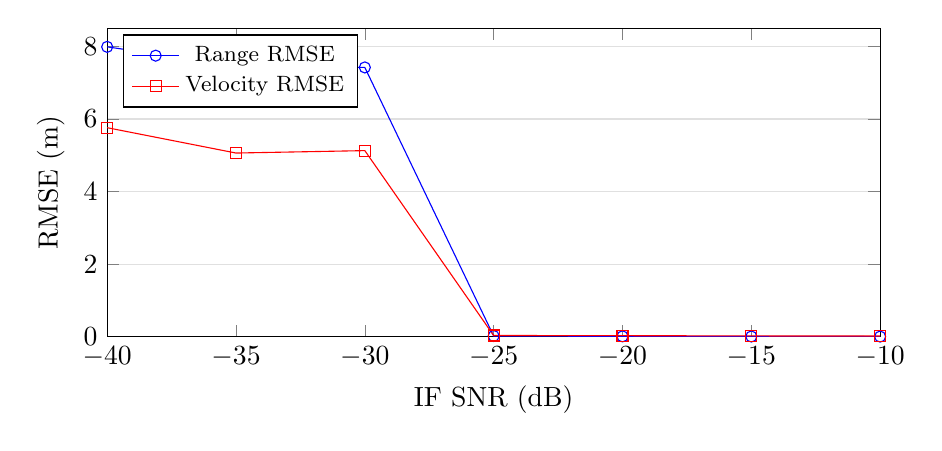
\begin{tikzpicture}
\begin{axis}[
width=0.94\textwidth,height=5.5cm,
xlabel={IF SNR (dB)},ylabel={RMSE (m)},
xmin=-40,xmax=-10,ymin=0,ymax=8.5,
legend style={font=\footnotesize,at={(0.02,0.98)},anchor=north west},
ymajorgrids=true,grid style={black!12}]
\addplot+[mark=o] coordinates {(-40,7.98657)(-35,7.46960)(-30,7.41971)(-25,0.02142)(-20,0.01151)(-15,0.00785)(-10,0.00560)};
\addplot+[mark=square] coordinates {(-40,5.75981)(-35,5.06158)(-30,5.12805)(-25,0.03511)(-20,0.03011)(-15,0.02290)(-10,0.02071)};
\legend{Range RMSE,Velocity RMSE}
\end{axis}
\end{tikzpicture}
\caption{Parking-profile pilot sensing evidence at $(R,v)=(10\,\mathrm{m},3\,\mathrm{m/s})$, 50 trials per SNR point. The sharp improvement around $-25$ dB is simulation evidence from the repository, not a hardware measurement.}
\label{fig:p1pilot}
\end{figure*}%
}
